%\documentclass{midl} % Include author names
\documentclass[anon]{midl} % Anonymized submission

% The following packages will be automatically loaded:
% jmlr, amsmath, amssymb, natbib, graphicx, url, algorithm2e
% ifoddpage, relsize and probably more
% make sure they are installed with your latex distribution

\usepackage{mwe} % to get dummy images
\jmlrvolume{-- Under Review}
\jmlryear{2024}
\jmlrworkshop{Full Paper -- MIDL 2024 submission}
\editors{Under Review for MIDL 2024}

\title[Innovative Cancer Cell Detection]{Innovative Cancer Cell Detection from Partial Annotations in Histopathology via Semi-supervised Learning}

 % Use \Name{Author Name} to specify the name.
 % If the surname contains spaces, enclose the surname
 % in braces, e.g. \Name{John {Smith Jones}} similarly
 % if the name has a "von" part, e.g \Name{Jane {de Winter}}.
 % If the first letter in the forenames is a diacritic
 % enclose the diacritic in braces, e.g. \Name{{\'E}louise Smith}

 % Two authors with the same address
 % \midlauthor{\Name{Author Name1} \Email{abc@sample.edu}\and
 %  \Name{Author Name2} \Email{xyz@sample.edu}\\
 %  \addr Address}

 % Three or more authors with the same address:
 % \midlauthor{\Name{Author Name1} \Email{an1@sample.edu}\\
 %  \Name{Author Name2} \Email{an2@sample.edu}\\
 %  \Name{Author Name3} \Email{an3@sample.edu}\\
 %  \addr Address}


% Authors with different addresses:
% \midlauthor{\Name{Author Name1} \Email{abc@sample.edu}\\
% \addr Address 1
% \AND
% \Name{Author Name2} \Email{xyz@sample.edu}\\
% \addr Address 2
% }

%\footnotetext[1]{Contributed equally}

% More complicate cases, e.g. with dual affiliations and joint authorship
\midlauthor{\Name{Author Name1\midljointauthortext{Contributed equally}\nametag{$^{1,2}$}} \Email{abc@sample.edu}\\
\addr $^{1}$ Address 1 \\
\addr $^{2}$ Address 2 \AND
\Name{Author Name2\midlotherjointauthor\nametag{$^{1}$}} \Email{xyz@sample.edu}\\
\Name{Author Name3\nametag{$^{2}$}} \Email{alphabeta@example.edu}\\
\Name{Author Name4\midljointauthortext{Contributed equally}\nametag{$^{3}$}} \Email{uvw@foo.ac.uk}\\
\addr $^{3}$ Address 3 \AND
\Name{Author Name5\midlotherjointauthor\nametag{$^{4}$}} \Email{fgh@bar.com}\\
\addr $^{4}$ Address 4
}

\begin{document}

\maketitle

\begin{abstract}
In this study, we introduce a streamlined semi-supervised approach that effectively leverages partially annotated datasets in histopathological images. We assessed three leading object detection models—YOLOv8s, Faster R-CNN, and YOLOv5s—ultimately selecting YOLOv8s for its superior capability in augmenting our dataset with pseudo labels. This approach markedly diminishes the need for exhaustive manual annotations, as YOLOv8s, combined with precise patch extraction and data augmentation, meticulously preserves essential cellular details in high-resolution images from Papillary urothelial carcinoma patients. Notably, YOLOv8s outperformed in terms of precision, recall, and computational efficiency, proving its adaptability across varied cancer types. After enriching our training with pseudo labels, we further refined our model and validated it on a fully annotated dataset, ensuring its robustness and precision. Despite the challenges of sparse annotations, our results underscore the efficacy of our semi-supervised model and emphasize the critical role of balanced annotation strategies. This study advances cancer diagnostics by introducing sophisticated object detection methodologies and sets a new precedent in medical image analysis, effectively navigating the constraints of limited annotated data with semi-supervised learning.
\end{abstract}

\begin{keywords}
Semi-supervised Learning, Cancer Cell Detection, Histopathological Imaging, YOLOv8s Model, Computational Pathology
\end{keywords}



\section{Introduction}

The integration of deep learning into medical imaging and pathology has sparked significant advancements in disease diagnosis and treatment strategies. In particular, the practice of knowledge distillation and the development of advanced object detection methodologies have been pivotal in enhancing the precision of cancer cell detection, a critical aspect of pathology \cite{Hinton:arXiv:2015:Distilling, Smith2018, Johnson2020}. Despite these advancements, the field continues to face challenges, especially concerning the efficient handling of datasets with varying levels of annotations and the intricate task of cell segmentation and classification in histopathological images.

In response to the need for improved object detection methods, several innovative approaches have been introduced. The study by Abbasi et al. proposed enhancing YOLO's performance on partially labeled datasets by creating pseudo-labels for unlabeled instances, significantly improving generalization performance \cite{abbasi2020self}. Similarly, the Co-mining approach adopted a self-supervised learning technique using a Siamese network for object detection in sparsely annotated settings \cite{wang2021co}. Niemeijer et al. further extended this concept by proposing a method for fusing datasets with partially overlapping classes, employing pseudo-labeling with uncertainty quantification to enhance model robustness \cite{niemeijer2023approach}.

The necessity for efficient data annotation has also led to the development of weakly supervised learning frameworks. Qu et al. introduced a novel framework for deep nuclei segmentation using partial points annotation, significantly reducing the annotation workload and enabling efficient large-scale medical image analysis \cite{qu2020weakly}. Complementing this, Greenwald et al. developed Mesmer, a deep learning algorithm for whole-cell segmentation in tissue images, which achieved human-level performance and addressed the critical challenge of cell segmentation in tissue imaging \cite{greenwald2022whole}.

In the realm of cell classification, groundbreaking advancements have been made by Amitay et al. with the development of CellSighter, a neural network demonstrating over 80\% accuracy in cell type classification from highly multiplexed images \cite{amitay2023cellsighter}. Similarly, Bortolomeazzi et al. introduced SIMPLI, a versatile tool for multiplexed image analysis, aligning perfectly with objectives to process complex histopathological images for accurate cancer cell detection \cite{bortolomeazzi2022simpli}.

However, these advancements are not without limitations. The challenge of handling long-tailed distributions in datasets, a common issue in cancer cell detection due to the diverse and imbalanced nature of histopathological datasets, was addressed by Zang et al. through the development of CascadeMatch \cite{zang2023semi}. Additionally, the need for efficient utilization of limited labeled data in medical image analysis led to the development of an end-to-end framework by Xu et al., harnessing unlabeled data effectively \cite{xu2021end}.

Significant contributions have also been made in the precise detection and classification of nuclei in histology images. Hover-Net, introduced by Graham et al., uniquely predicts distances of nuclear pixels to their centers, enabling accurate segmentation, and classifies each nucleus type, integrating segmentation and classification tasks \cite{graham2019hover}. Moreover, Schmidt et al. presented StarDist, a novel method for cell detection in microscopy images, utilizing star-convex polygons for segmentation and effectively handling crowded cellular environments \cite{schmidt2018cell}.

In addressing the challenges of time-consuming human labeling and the complex nature of pathology images, which may contain thousands of cells, our work introduces a semi-supervised learning approach for creating pseudo labels. Initially, we trained three networks on partially annotated datasets. Subsequently, we selected the best-performing network based on its performance metrics on the partially annotated data. Our method involves first training the most effective detector network, as identified in the previous stage, using partial annotations. Then, we employ the pseudo labels generated by the learned model to retrain a new detector. This innovative approach not only addresses the inefficiencies in human labeling but also leverages the strengths of semi-supervised learning to enhance the model's performance. Furthermore, we conducted a comprehensive comparison of our method's performance across different portions of annotations. To validate our pipeline, we meticulously tested it with five different types of cancer, each fully annotated by professional pathologists. This rigorous validation underscores the robustness and effectiveness of our approach, setting a new precedent in the field of medical image analysis and pathology.

\section{Methodology}
\label{sec:methodology}

\subsection{Introduction to Methodology and Iterative Training Approach}
This study delves deeply into medical image analysis, focusing on evaluating the performance of leading object detection models: YOLOv8s \cite{ultralytics2023}, Faster R-CNN \cite{ren2015faster}, and YOLOv5s \cite{yolov5}. These models are meticulously assessed for their proficiency in detecting and classifying cancer cells within histopathological images, a process integral to advancing the precision and speed of object detection, pivotal factors in the early and accurate diagnosis of cancer.

In this exploration, an iterative training approach is adopted. Initially, all detectors are trained on partially annotated datasets, a strategy that addresses the challenges associated with extensive manual annotations. Subsequently, the best-performing detector, as determined by the comparative analysis, is selected to generate pseudo labels. These pseudo labels are then used to retrain a new detector, enhancing the model's learning process and improving its detection capabilities. This methodological evolution is graphically depicted in Figure~\ref{fig:1}, which provides a schematic explanation of our proposal for generating pseudo-labels and employing a semi-supervised learning approach with the YOLOv8s model for the detection of cancer cells, including CD45, panCK, and others.

\begin{figure}[htbp]
\floatconts
{fig:1}
{\caption{Schematic explanation of our proposal for generating pseudo-labels and utilizing a semi-supervised learning approach with the YOLOv8s model for the detection of fully cancer cells, including CD45, panCK, and others.}}
{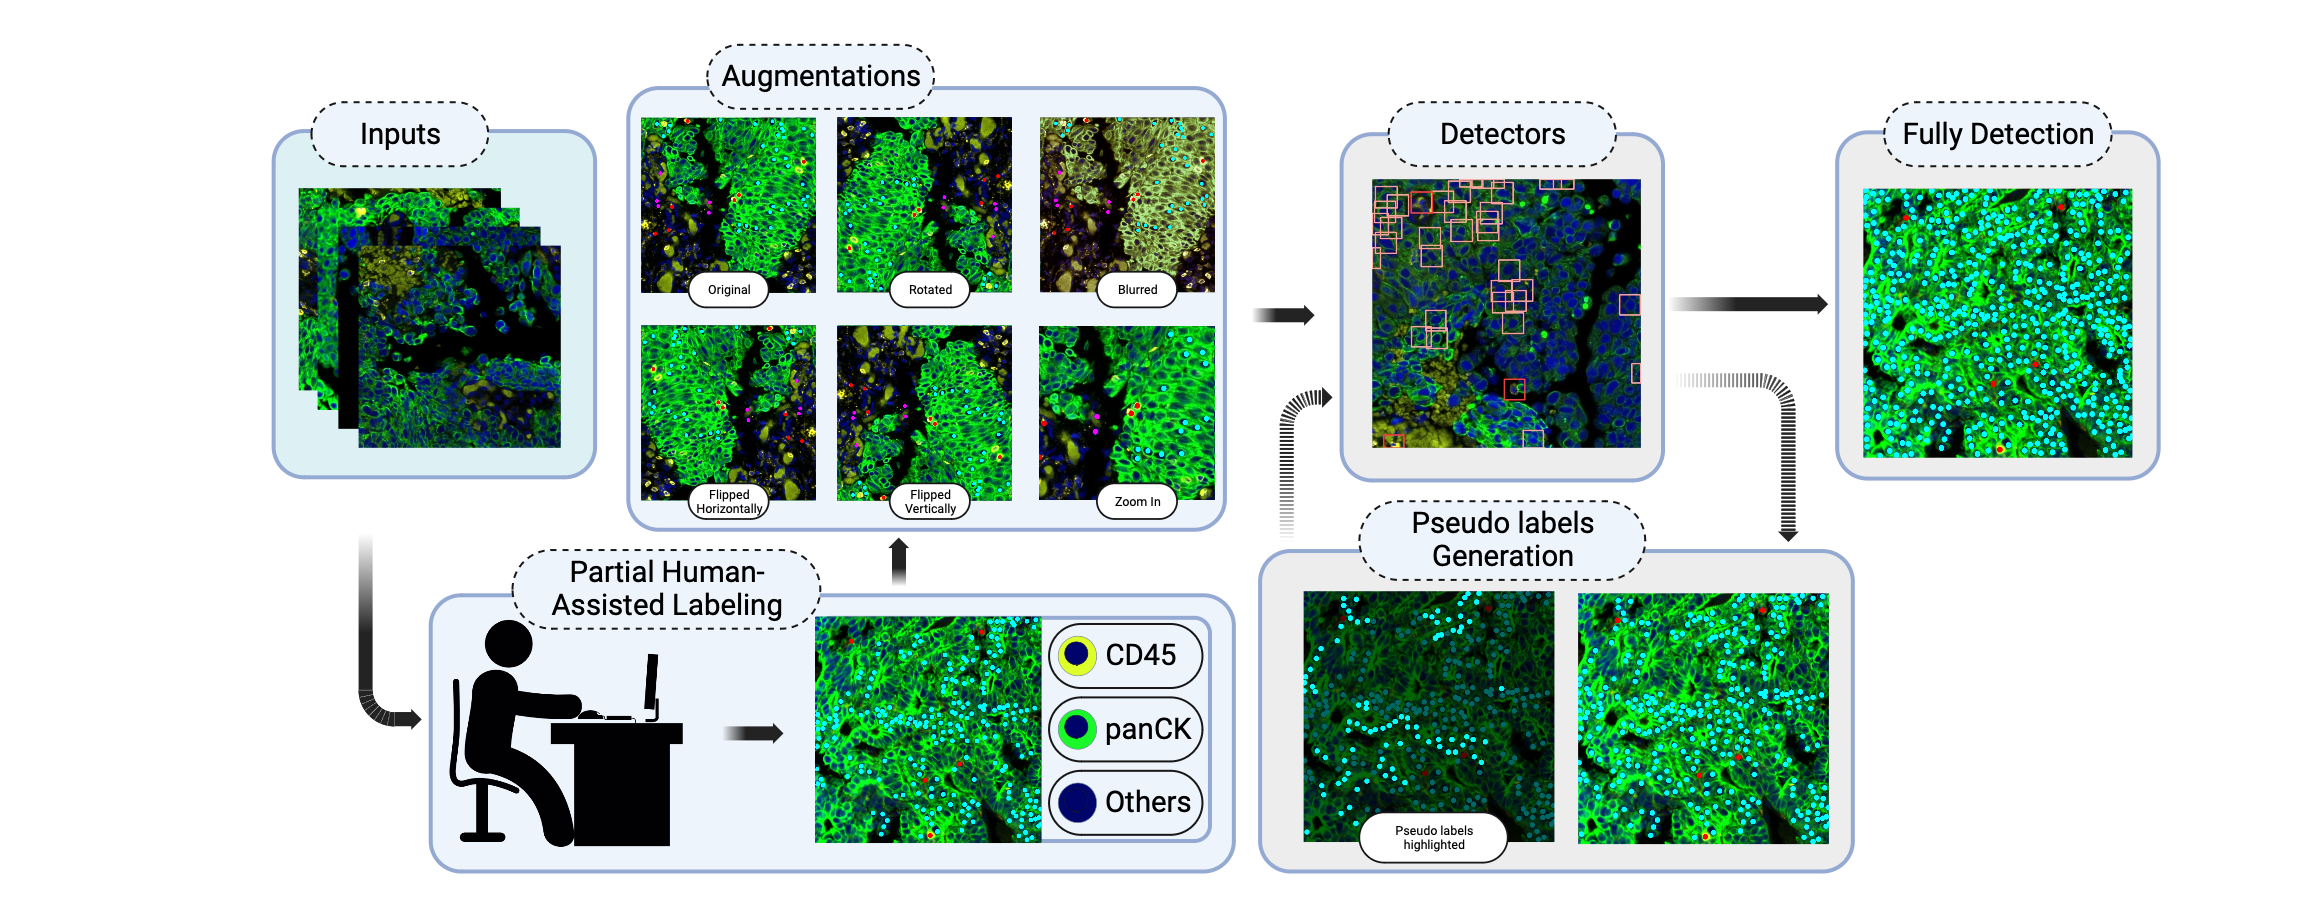
\includegraphics[width=1\linewidth]{images/1.png}}
\end{figure}

\subsection{Data Collection, Preparation, and Annotation Strategy}
This study utilizes a dataset consisting of high-resolution histopathological images from patients with Papillary urothelial carcinoma, featuring 10 images in total. Of these, 8 are allocated for training the detectors, while the remaining 2 are reserved for testing. To manage the extensive size of these images, a patch extraction method was applied, creating sections of 640x640 pixels that retain essential cellular features critical for accurate detection (Figure~\ref{fig:2}).

The dataset was further enriched through data augmentation techniques such as flipping, zooming, rotating, and blurring, expanding the dataset to 51,924 patches, of which 9,880 are used for testing. This process not only diversifies the imaging conditions but also enhances the robustness of the models in detecting cancer cells under various scenarios.

Recognizing the labor-intensive nature of annotating large histopathological images, the study employed a partial annotation strategy. Here, experienced pathologists annotated approximately 10\% of the cells in the images, striking a balance between manual annotation efforts and the need for accurately labeled data for model training.


\begin{figure}[htbp]
\floatconts
{fig:2}
{\caption{Overview of the Dataset Showcasing Cell Type Shapes, the Number of Initial Annotations per Class, and Fully Annotated Cancer Types for Validation.}}
{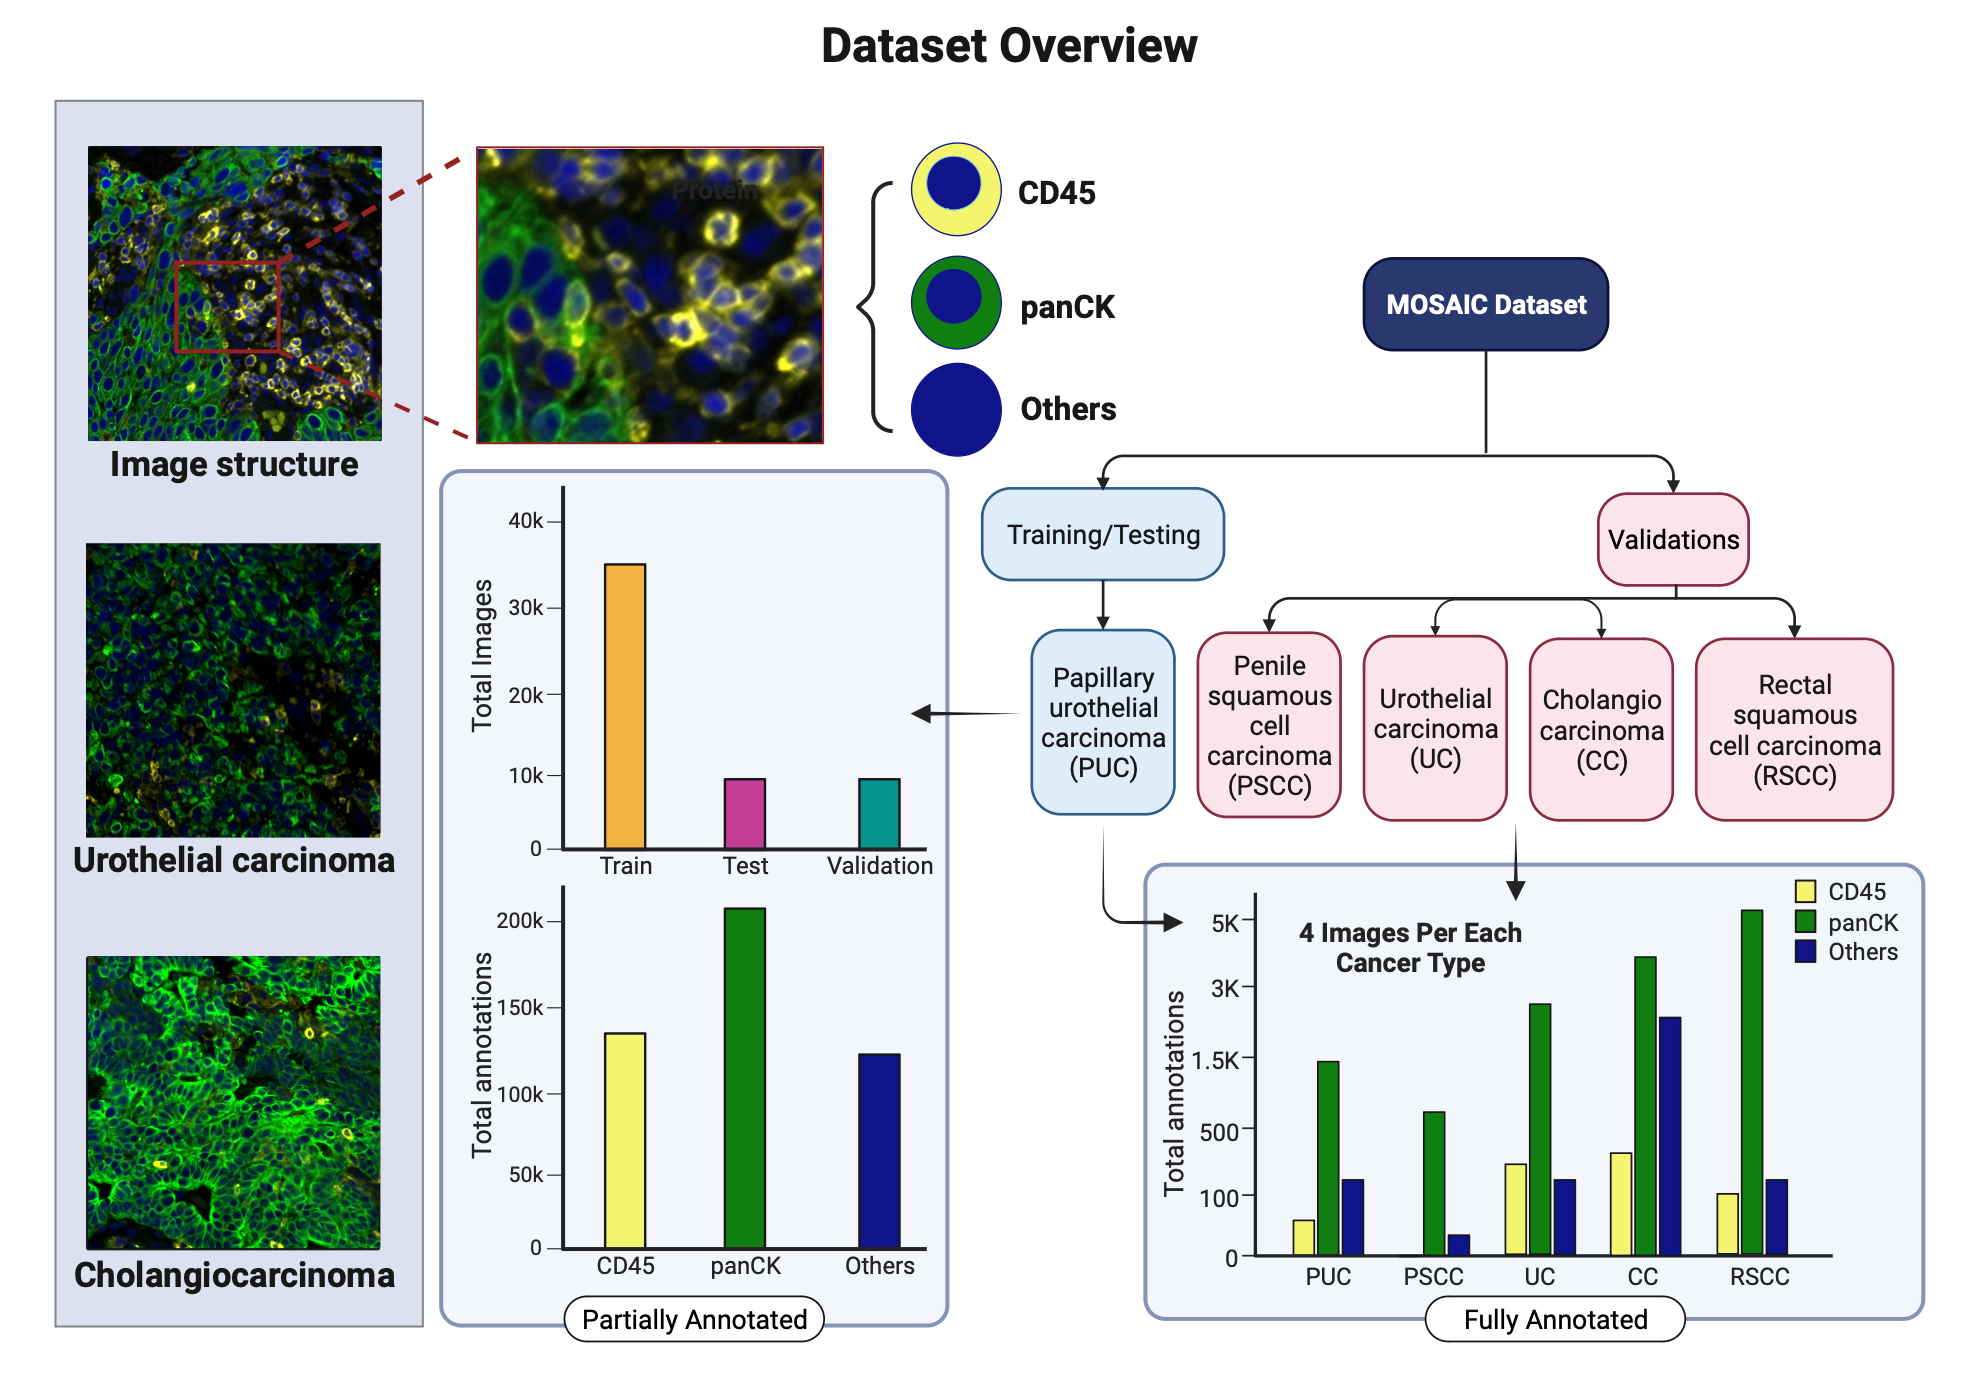
\includegraphics[width=1\linewidth]{images/2.png}}
\end{figure}


\subsection{Model Training, Pseudo Label Generation, and Validation}

The initial training phase involved pretraining the YOLOv8s model with partially annotated data, guided by semi-supervised object detection strategies to effectively utilize a limited number of labeled images \cite{gao2019note, jeong2019consistency}. This approach helps control overfitting, a challenge in models trained on sparsely annotated datasets. Subsequently, the model was retrained to generate pseudo labels, drawing from methods like CSD \cite{jeong2019consistency} that apply consistency constraints to maximize the use of unlabeled data. These pseudo labels, when integrated with the initial annotations, enriched the training dataset and enhanced the model's capability to detect various cellular entities accurately.

During validation and testing, the models' adaptability and robustness were thoroughly assessed across diverse cancer types and annotation levels. Evaluation metrics such as accuracy, precision, recall, mAP50, and F1-score provided a comprehensive understanding of the models' performance. Furthermore, the study incorporated additional fully annotated datasets of various cancer types for validation, enriching the robustness and adaptability of the models to different cancer cell appearances and histopathological conditions,  as depicted in Figure~\ref{fig:2}.

This streamlined approach, combining semi-supervised learning with iterative training and thorough validation, not only refines cancer cell detection in histopathological imaging but also sets the stage for future advancements in medical image analysis, demonstrating the potential of leveraging partially annotated datasets for efficient and precise diagnostics.



\section{Results}
\subsection{Initial Phase: Selection of Best Object Detection Model}
This section encapsulates the comparative performance analysis of various object detection networks, with a specific focus on their capabilities in identifying distinct cancer cell types. The initial phase of our study involved training three distinct networks (YOLOv8s, Faster RCNN, and YOLOv5s) on a dataset that was partially annotated. Post the initial training phase, we meticulously evaluated the performance of these models, ultimately selecting YOLOv8s for further processes based on its superior performance metrics.

After the initial stage, we used YOLOv8s to create additional training data (pseudo labels) and added these to our original dataset to improve our model further. This method, which involves a semi-supervised learning and a step-by-step refinement process, greatly improved the model's ability to correctly identify cancer cells. The effectiveness and details of our approach are clearly shown and explained in Figure~\ref{fig:2}.

Table~\ref{tab:comparison_results} provides a detailed comparison of the object detection models, showcasing the outstanding performance of YOLOv8s in accurately detecting different types of cancer cells. The table presents key measures of model performance—precision, recall, and mAP50. YOLOv8s achieved excellent precision and mAP50 scores (0.99) for all types of cells, and its recall scores were consistently high, ranging from 0.97 to 0.98. In contrast, Faster R-CNN showed lower performance, with its precision, recall, and mAP50 scores varying more widely across different cell types. YOLOv5s, however, performed similarly to YOLOv8s, with high precision and mAP50 scores and competitive recall scores. These results clearly highlight YOLOv8s's superior ability to detect cancer cells, marking a significant improvement in accuracy and reliability compared to other models.

\begin{table}[htbp]
\floatconts
  {tab:comparison_results}%
{\caption{Performance Comparison of Object Detection Networks across Cell Types, Trained on an Initially Partially Annotated Dataset with 250 Epochs.}}%
  {\begin{tabular}{l|ccc|ccc|ccc}
  \bfseries Metric & \multicolumn{3}{c|}{\bfseries YOLOv8s} & \multicolumn{3}{c|}{\bfseries Faster RCNN} & \multicolumn{3}{c}{\bfseries YOLOv5s}\\
  & {\small \bfseries CD45} & {\small \bfseries panCK} & {\small \bfseries Others} & {\small \bfseries CD45} & {\small \bfseries panCK} & {\small \bfseries Others} & {\small \bfseries CD45} & {\small \bfseries panCK} & {\small \bfseries Others}\\
  Precision & 0.99 & 0.99 & 0.99 & 0.88 & 0.85 & 0.83 & 0.99 & 0.99 & 0.99\\
  Recall & 0.97 & 0.97 & 0.98 & 0.85 & 0.82 & 0.80 & 0.96 & 0.98 & 0.96\\
  mAP50 & 0.99 & 0.99 & 0.99 & 0.84 & 0.81 & 0.79 & 0.98 & 0.98 & 0.98
  \end{tabular}}
\end{table}

\subsection{Annotation Impact: Analyzing Model Performance at Different Annotation Levels}
Given the superior performance of YOLOv8s in detecting cancer cells, as evidenced in Table~\ref{tab:comparison_results}, we further investigated its robustness under varying annotation scenarios. Specifically, we evaluated the model's performance when trained with different proportions of annotated data: 100\%, 50\%, and 25\%. The outcomes of this experiment, detailed in Table~\ref{tab:annotation_comparison}, provide insight into the minimum level of annotations required to maintain acceptable detection results.

As depicted in Table~\ref{tab:annotation_comparison}, YOLOv8s maintains respectable performance metrics with a full annotation set (100\%). However, a notable decrease in precision, recall, and mAP50 is observed as the level of annotations is reduced. With 50\% annotations, the model achieves a precision of 0.72 and a recall of 0.74, alongside a mAP50 of 0.79, indicating a moderate decline in performance. The impact is more pronounced at 25\% annotations, where precision drops to 0.19, recall to 0.51, and mAP50 to 0.18, suggesting a significant compromise in the model's detection capabilities.It's important to note that our strategy for reducing annotations was methodical. We ensured an even distribution of annotations across different cell types, rather than removing them randomly. This approach was intended to maintain a balanced representation of each cell type in the training data.

These findings highlight the importance of a sufficient quantity of annotations for training robust deep learning models like YOLOv8s. While the model demonstrates a certain degree of tolerance to reduced annotations, ensuring a higher percentage of annotated data is imperative for optimal performance, especially in the critical domain of cancer cell detection.

\begin{table}[htbp]
\floatconts
  {tab:annotation_comparison}%
  {\caption{YOLOv8s Performance with Varying Annotation Levels (250 epochs.)}}%
  {\begin{tabular}{lccc}
  \bfseries Metric & \bfseries 100\% Annotations & \bfseries 50\% Annotations & \bfseries 25\% Annotations\\
  Precision & 0.98 & 0.72 & 0.19\\
  Recall & 0.97 & 0.74 & 0.51\\
  mAP50 & 0.99 & 0.79 & 0.18
  \end{tabular}}
\end{table}

\subsection{Final Phase: Pseudo Label Integration and Validation on Fully Annotated Dataset}
In the final stage, we enhanced YOLOv8s by integrating pseudo labels with the original dataset, a process that involves semi-supervised learning and iterative refinement. This strategy significantly improved the model's ability to detect cancer cells.  In this validation study, for each cancer type, we used four patches of size 640x640 pixels, which were fully annotated by two pathologists. Figure~\ref{fig:cc_comparison} exemplifies one such annotated patch from the Cholangiocarcinoma (CC) cancer type, illustrating the comparison between the expert pathologists' annotations and the predictions made by YOLOv8s. This detailed annotation provided a robust basis for evaluating the YOLOv8s model's performance. The comprehensive validation of the YOLOv8s model across various cancer types is  presented in Table~\ref{tab:cancer_validation}, underscoring the model's robustness and adaptability. The model was tested against five distinct cancer types, namely Papillary Urothelial Carcinoma (PUC), Penile Squamous Cell Carcinoma (PSCC), Urothelial Carcinoma (UC), Cholangiocarcinoma (CC), and Rectal Squamous Cell Carcinoma (RSCC). Notably, YOLOv8s demonstrated high precision (P), recall (R), and F1 Score across all cancer types, affirming its competence in handling diverse histopathological scenarios.

\begin{figure}[htbp]
\floatconts
  {fig:cc_comparison}
  {\caption{Comparison of Cholangiocarcinoma (CC) cell detection between Pathologist annotations and YOLOv8s predictions. The left panel shows the patch fully annotated by pathologists, while the right panel displays YOLOv8's detections. Red dots represent CD45 cells, cyan dots represent panCK cells, and magenta dots indicate Other cell types. The numbers at the bottom denote the count of each cell type.}}
  {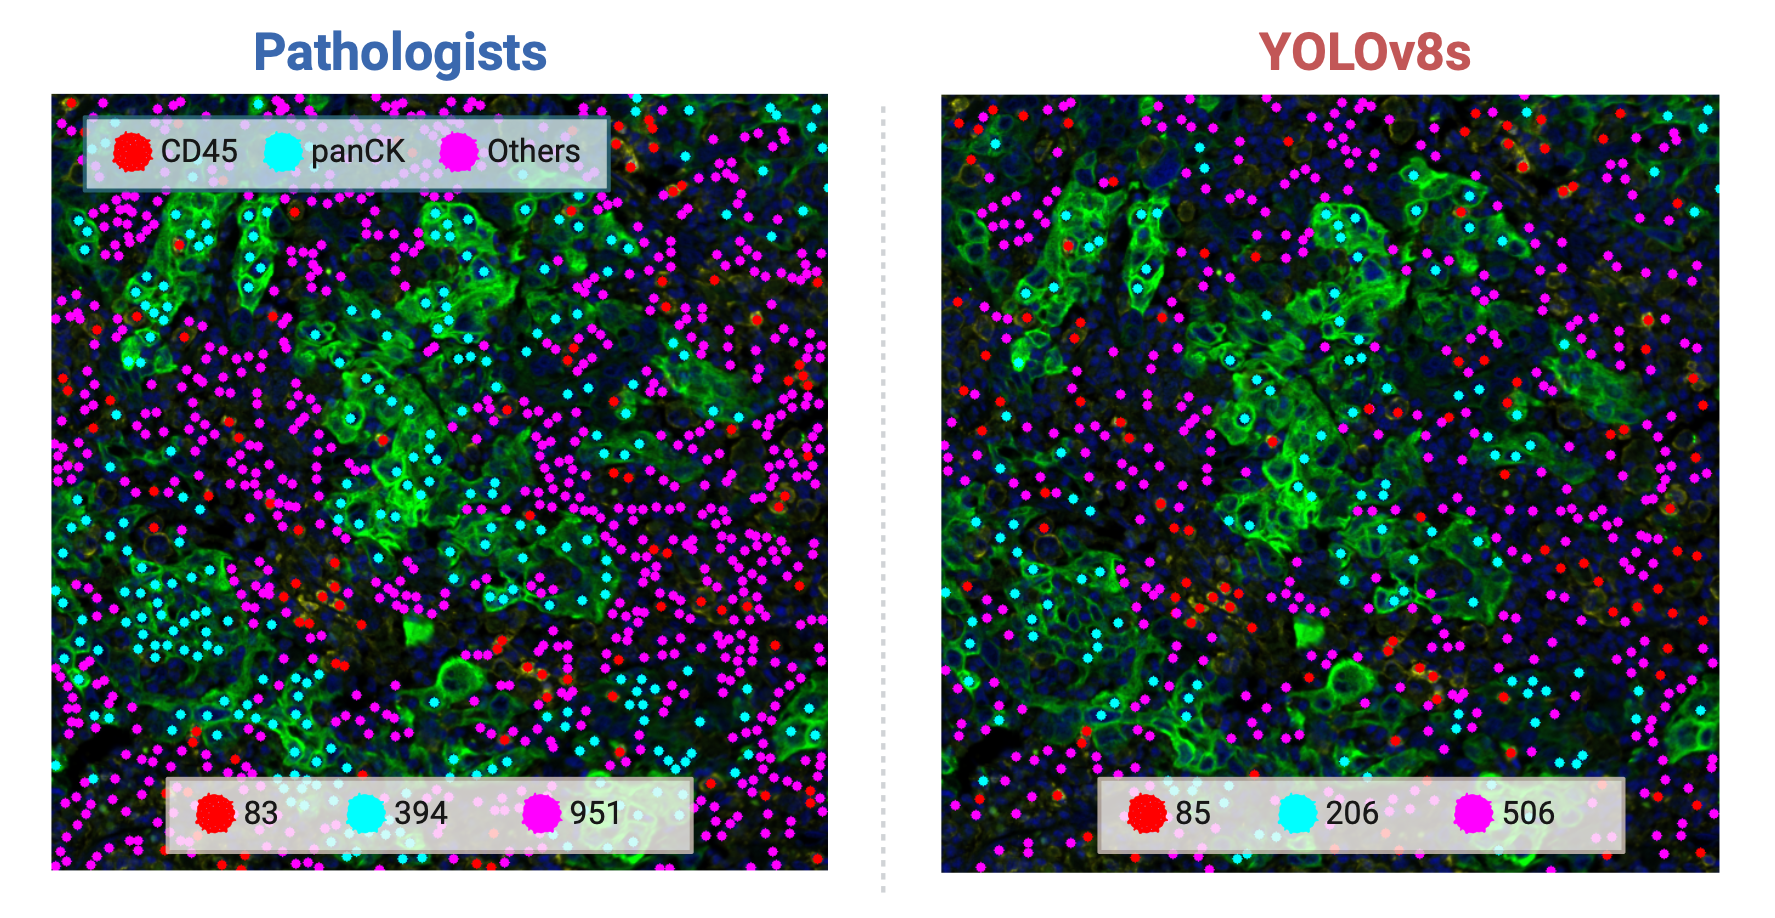
\includegraphics[width=1\linewidth]{images/3.png}}
\end{figure}

For PUC, the model achieved a precision of 100.0\% and recall of 68.0\%, with an F1 Score of 78.9\%. In the challenging PSCC samples, the model maintained a precision of 65.9\% and recall of 74.6\%, reflecting its effectiveness despite the lower precision in comparison to other types. UC samples, showcasing a balance in the distribution of cells, exhibited outstanding model performance with a precision of 82.1\% and a recall of 81.9\%. In the context of CC and RSCC, which presented lower cell counts and varied cell distribution, YOLOv8 demonstrated its versatility and accuracy, sustaining high validation metrics: precision of 97.7\% and recall of 72.9\% for CC, and precision of 98.3\% and recall of 63.6\% for RSCC. The consistent performance metrics across various cancer types underline the potential of YOLOv8 as a reliable tool in digital pathology, promising significant strides towards automated and precise cancer diagnostics.


\begin{table}[htbp]
\floatconts
  {tab:cancer_validation}%
  {\caption{Validation Metrics of YOLOv8s on Various Cancer Types. The cancer types are indicated as: PUC (Papillary Urothelial Carcinoma), PSCC (Penile Squamous Cell Carcinoma), UC (Urothelial Carcinoma), CC (Cholangiocarcinoma), RSCC (Rectal Squamous Cell Carcinoma).}}%
  {\begin{tabular}{l|ccc|ccc|ccc}
  \bfseries Type & \multicolumn{3}{c|}{\bfseries Path. Count} & \multicolumn{3}{c|}{\bfseries YO8 Count} & \multicolumn{3}{c}{\bfseries Metrics (\%)}\\
  & \bfseries CD45 & \bfseries panCK & \bfseries Oth & \bfseries CD45 & \bfseries panCK & \bfseries Oth & \bfseries P & \bfseries R & \bfseries F1\\
  PUC & 47.5 & 707 & 83 & 39.75 & 272 & 68 & 100.0 & 68.0 & 78.9\\
  PSCC & 0 & 313 & 11 & 0 & 154 & 34.5 & 65.9 & 74.6 & 57.2\\
  UC & 47.5 & 703.5 & 32 & 39.75 & 437 & 69.25 & 82.1 & 81.9 & 77.0\\
  CC & 37.14 & 522.71 & 300 & 39.86 & 326 & 168.86 & 97.7 & 72.9 & 81.8\\
  RSCC & 47.5 & 2629.5 & 59 & 50 & 1162.5 & 27.5 & 98.3 & 63.6 & 74.1
  \end{tabular}}
\end{table}


\section{Discussion}

\subsection{Interpretation of Results}
The outcomes of this study underscore the potential of the YOLOv8s model in revolutionizing cancer cell detection through histopathological imaging. The model's exemplary performance, reflected in the high precision, recall, and mAP50 scores across various cancer cell types, attests to its robustness and accuracy. YOLOv8's ability to outperform established models like Faster R-CNN and YOLOv5, particularly in the context of precision and mAP50, highlights the advanced capabilities of this deep learning approach. The nuanced detection of cell types such as CD45, panCK, and others, is indicative of the model's intricate understanding of morphological characteristics, a crucial factor in the precise identification and classification of cancer cells.

The model's validation on fully annotated patches across a variety of cancer types, despite being trained on a dataset with partial annotations (approximately 10\% of full annotations), not only underscores its capability to detect the majority of cells within the patches but also demonstrates its versatility in addressing different cancer types. This adaptability and reliability are evident in the consistent performance across various histopathological conditions, ranging from Papillary Urothelial Carcinoma to Rectal Squamous Cell Carcinoma.

The model's proficiency, as seen in these diverse scenarios, echoes the insights of Amitay et al., who highlighted the importance of precise cell classification in computational pathology \cite{amitay2023cellsighter}. Furthermore, the ability of YOLOv8s to deliver high performance, even with a limited set of annotations, is indicative of its robust learning mechanism and its capacity to generalize from sparse data. This characteristic is particularly valuable considering the resource-intensive nature of manual annotations in medical imaging, a challenge also acknowledged in the work of Qu et al. \cite{qu2020weakly}. This robustness and adaptability make our model a promising tool in the field of digital pathology, opening new avenues for efficient and accurate cancer cell detection and classification.

\subsection{Limitations, Future Work, and Broader Implications}

While the study presents promising results, certain limitations and opportunities for future research are apparent. The observed decrease in model performance with reduced annotations, especially below the 25\% threshold, underscores the need for an optimal balance between computational efficiency and the availability of annotated data. Future endeavors could focus on refining the model's performance under sparse annotations, potentially employing advanced semi-supervised learning techniques, as highlighted by Xu et al. \cite{xu2021end}. Furthermore, extending the model's detection capabilities to encompass a broader range of cell types and pathological conditions could offer a more holistic tool for pathologists, possibly integrating with comprehensive analysis software like SIMPLI, as suggested by Bortolomeazzi et al. \cite{bortolomeazzi2022simpli}.

The broader implications of this research signify its potential impact beyond cancer cell detection. The adaptability and efficacy of the YOLOv8s model hint at its applicability in various sectors of medical imaging and diagnostics. Its proficiency in processing complex histopathological images can significantly contribute to digital pathology and computational oncology, potentially expediting and refining cancer diagnoses. Furthermore, incorporating such sophisticated deep learning models into healthcare systems is in line with the overarching goal of AI in healthcare: to enhance diagnostic precision and elevate patient outcomes.

In essence, this study enriches the domain of medical image analysis with an advanced deep learning model for cancer cell detection and sets a trajectory for future research and practical applications. By navigating through the current limitations and exploring novel avenues, the full potential of YOLOv8s and similar models can be harnessed, heralding a new era in healthcare diagnostics.





% Acknowledgments---Will not appear in anonymized version
\midlacknowledgments{We thank a bunch of people. This work was supported by the MD Anderson Patient Mosaic™ Project at The University of Texas MD Anderson Cancer Center. Patient Mosaic is supported by generous philanthropic contributions from the Albert and Margaret Alkek Foundation, among others.}



\bibliography{midl-samplebibliography}



\end{document}
